\subsection{Integrated deduplication, caching, and Docker registries}
\label{sec:design}

%\sysname\ performs file-level deduplication for a Docker registry.
%
\begin{figure*}[t]
	\centering
		%\begin{minipage}{0.225\textwidth}
			\centering
			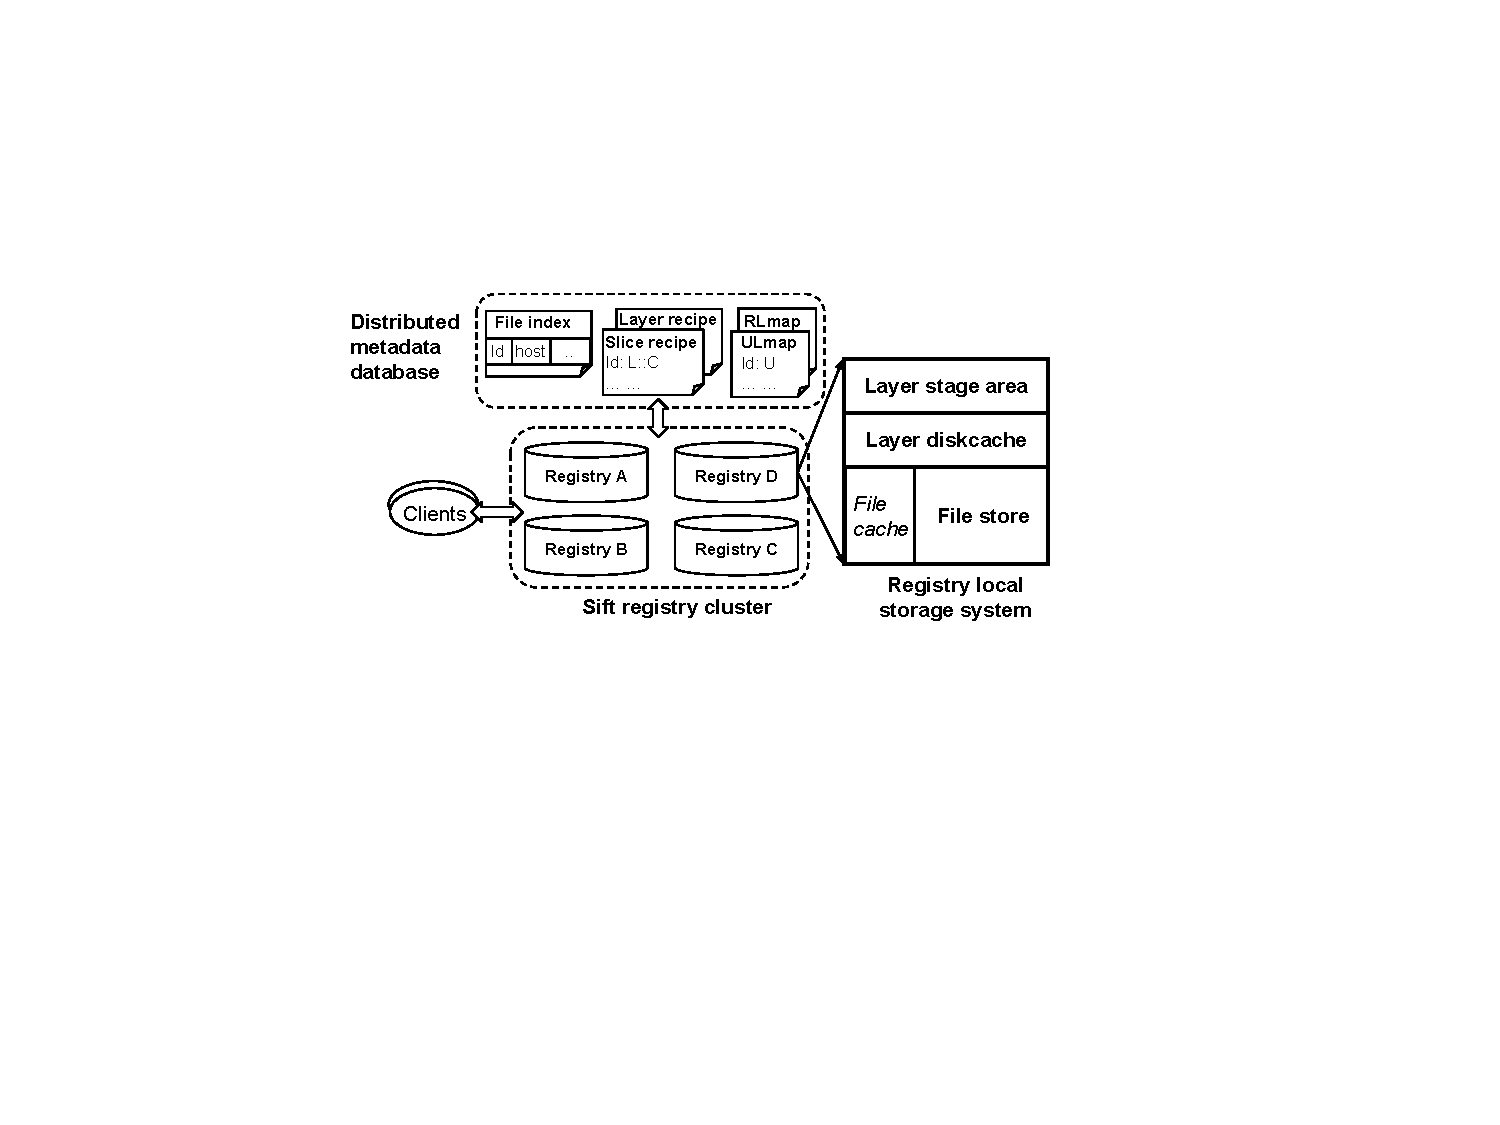
\includegraphics[width=0.9\textwidth]{graphs/sys-architecture.pdf}
%\vspace{-4pt}
			\caption{Architecture of \sysname.}
			%\label{fig:ref_count}
		%\end{minipage}
%	\begin{minipage}{0.225\textwidth}
%		\centering
%		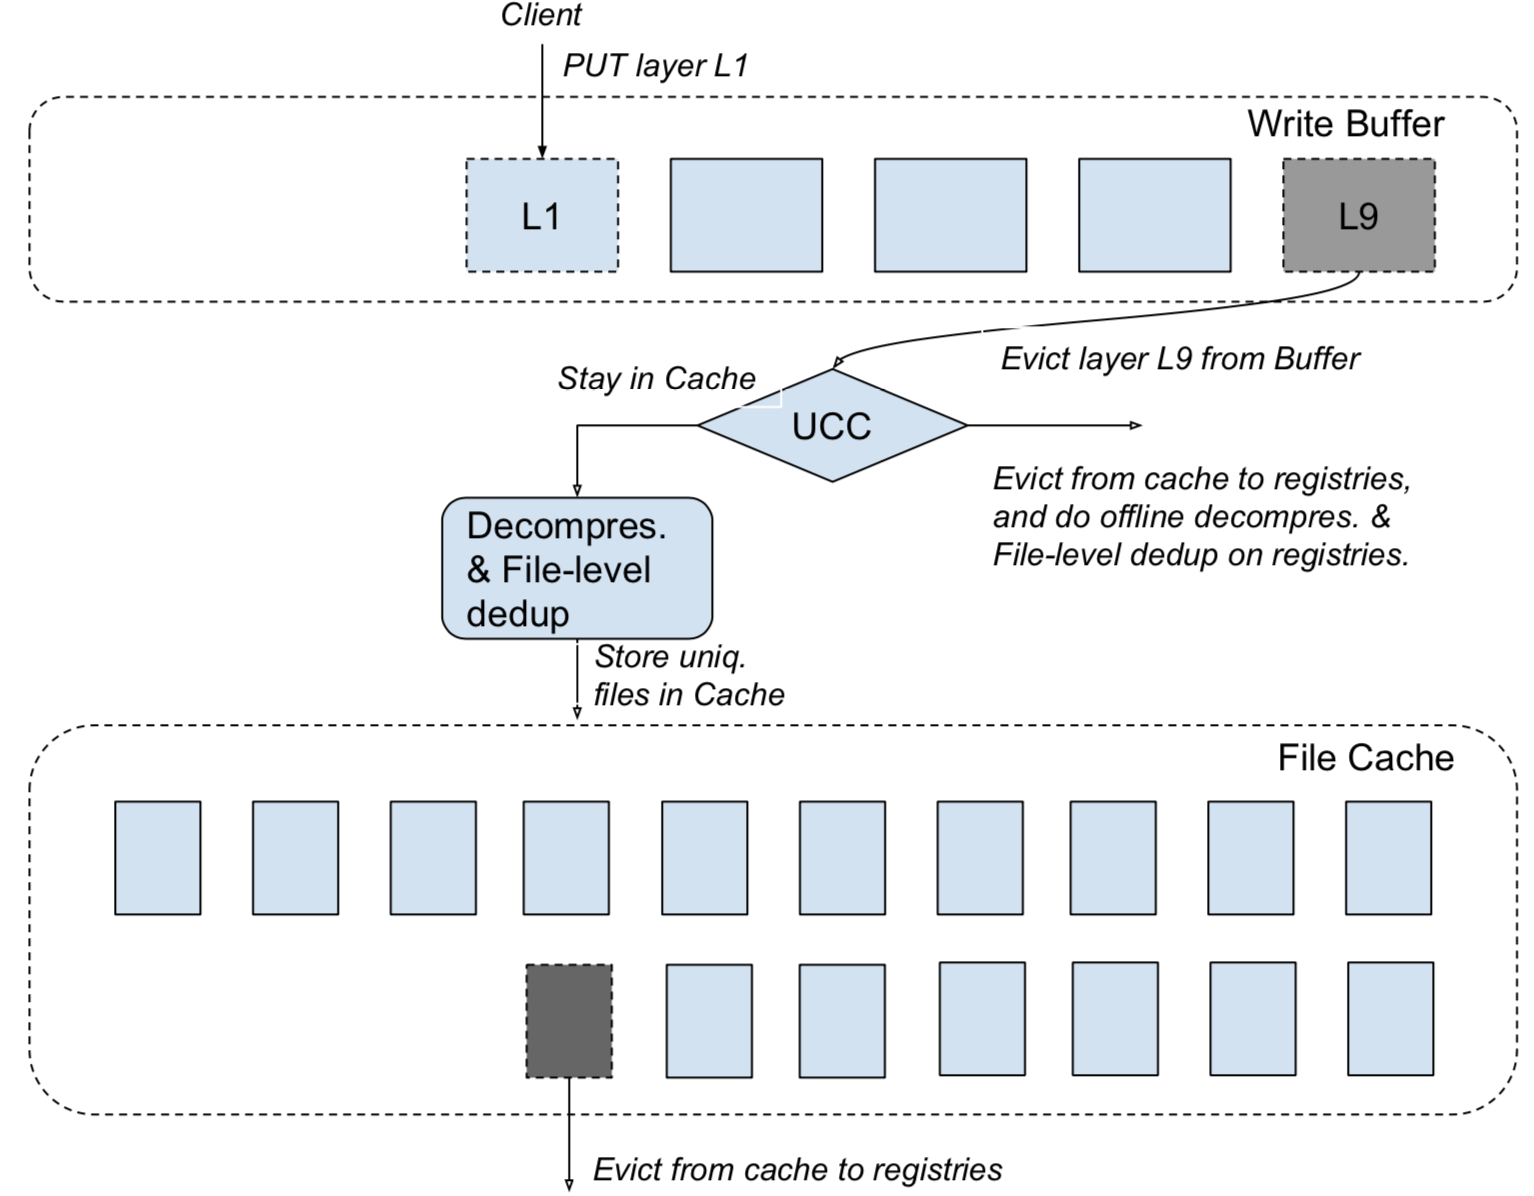
\includegraphics[width=1\textwidth]{graphs/slimmer-cache.png}
%		\caption{CDF of compress. and uncompress. layer size.}
%		\vspace{-3pt}
		\label{fig:sys-overview}
%\vspace{-4pt}
%	\end{minipage}
\end{figure*}

%We designed \sysname\ so that the interface between the Docker clients and the
%registry remains unchanged.
%
%As such, no modifications to the Docker clients are needed.
%
%Below we describe how \sysname\ handles layer pushes and
%pulls at the registry side.
%
%For the sake of this paper, we explain only the main steps omitting smaller
%details.

\sysname~seamlessly integrates the management of cache, deduplication on backend storage, and Docker registries,
and also redesign the key workflows required for each functionality. 
Traditionally, caches are placed as close to the requesting client as possible, such caches are known as proxy caches, or web/HTTP caches for the short-lived storage of 
frequently requested/accessed data to reduce the server's lag. 
They are typically implemented in an regional ISP or within a corporate network.
Deduplication methods are implemented on remote backend storage servers, and
transparently remove duplicates from the incoming data stream and restore the data for read requests. 
Docker registry is a web server that serves docker pull and docker push requests.
Although Docker registry is a layer-level content addressable storage system holding all the images,
it delegates storage to drivers which interact with either a local file system or a remote cloud storage like S3, Microsoft Azure, OpenStack Swift, and Aliyun OSS.
Intuitively, registries can be deployed as a proxy cache to host frequently requested layers to speedup image pulls and improve performance 
while the backend cloud storage can leverage deduplication to save storage space.
However, there are several unique problems concerning the integration of caching and deduplication to the unique Docker registries workload: layers. 

First, for caching layers, pull layer requests are difficult to predict because layer reuse time is very long. 
We observed that, on average, around half of layers' reuse time is longer than 4 hours which means 
that if we cache a layer, we might need to wait hours to get a hit on that layer.
This is because when a user pulls an image from registry, the Docker daemon on the requesting host will only pull the layers that are not stored locally. 
Moreover, we have to consider that users might deploy their applications on different machines, so it's not easy to predict 
when a user will access which layers.
Anwar et. al, proposed a prefetching method~\cite{anwarfast}: when there is a put layer request directly followed by a get manifest request, a get layer request will most probably follow.
However, based on our trace analysis, only half of pull layer requests have a precedent put layer request within the trace collecting period. Besides,
after a user pushes a layer to the repository, it takes a few days, weeks, or even months for a user to make a pull requests.
Second, for deduplicating compressed layers, the layers should first be decompressed then the uncompressed data undergoes a file-level deduplication. While for restoring a layer, the layer's
containing files should all be fetched from wherever they reside, as they are likely to be scattered across multiple servers, and compressed together, which causes a considerable overhead on pull layer requests performance.

To meet this challenge, we propose a new design featuring a user behavior based cache comprising a \emph{layer buffer} and a
\emph{file cache} to cache layers and cache unique files after decompression and deduplication, respectively.
This design considers user behavior, including when a user will be active later, which is decisive for layer evictions from the cache.
Based on our observation, user behavior is easier to predict as shown in Figure~\ref{reusetime}.
The layer buffer stores all the newly pushed layers in memory. 
Although accessing memory is very fast, the size of main memory is limited. 
Considering layer sizes around a few megabyte on average, a small main memory cache cannot accommodate many active users' layers.

To address this issue, we couple main memory cache and flash memory cache to provide separate caching for layers and unique files, respectively.
When handling cache evictions, we first evict inactive users' layers from the layer buffer to the file cache after performing 
the following operations: decompressing each evicted layer and comparing its containing files with the files that are already 
stored in the file cache, eliminating duplicate files, that is, only storing the unique files on flash storage.
Consequently, the flash memory cache is facilitating the logical accommodation of more layers when compared to only naively caching layers.
When a user requests a layer not present in the layer buffer, the request is forwarded to the file cache. 
More specifically, the request will be separately forwarded to all the servers that store its containing files. 
The servers compress the files individually and send partial layers back to the user. 
Here, we change the Docker client interface such that when it receives all the compressed parts of the layer, it can decompress them. 
Forwarding partial layers from servers in parallel eliminates the network latency caused by fetching files from different servers and assembling them into a whole compressed layer.
Furthermore, compressing partial layers in parallel considerably mitigates the compression latency caused by compressing a whole layer since compression time depends on the size of the uncompressed files.

    





 
